\documentclass[twocolumn]{article}

\usepackage{graphicx}
\usepackage{xeCJK}
\usepackage{bm}
\usepackage{amsmath,amsthm,amssymb,amsfonts}
\usepackage{cite}
\usepackage[colorlinks,linkcolor=red,anchorcolor=blue,citecolor=green,CJKbookmarks=true]{hyperref}
\usepackage{indentfirst}
\usepackage{amsmath}
\usepackage[margin=3.5cm]{geometry}
\usepackage{titlesec}
\usepackage{amsmath}
\usepackage{amssymb}
% \linespread{1.6}
\usepackage{multirow}
\usepackage{listings}
\usepackage{xcolor}
\usepackage{ulem}
\geometry{left=1.8cm,right=1.8cm,top=1.5cm,bottom=1.5cm}
\usepackage{enumitem}
\usepackage{tikz}
\usepackage{lipsum}
\setenumerate[1]{itemsep=0pt,partopsep=0pt,parsep=\parskip,topsep=5pt}
\setitemize[1]{itemsep=0pt,partopsep=0pt,parsep=\parskip,topsep=5pt}
\setdescription{itemsep=0pt,partopsep=0pt,parsep=\parskip,topsep=5pt}
%定理
\makeatletter
\thm@headfont{\sc}
\makeatother
\newtheorem{theorem}{Theorem}
%%%%%%%%%%%%% C++ Code
\usepackage{color}
\usepackage{xcolor}
\definecolor{keywordcolor}{rgb}{0.8,0.1,0.5}
\usepackage{listings}
\lstset{breaklines}%这条命令可以让LaTeX自动将长的代码行换行排版
\lstset{extendedchars=false}%这一条命令可以解决代码跨页时,章节标题,页眉等汉字不显示的问题
\lstset{ %用于设置语言为C++
    keywordstyle=\color{keywordcolor} \bfseries, 
    %identifierstyle=,
    basicstyle=\ttfamily, 
    commentstyle=\color{blue} \textit,
    stringstyle=\ttfamily, 
    showstringspaces=false,
    frame=shadowbox, %边框
    %captionpos=b
}

%\setCJKmainfont[BoldFont = 黑体]{宋体}
\setmainfont{Times New Roman}
\setsansfont{Helvetica}
\setmonofont{Courier New}
\setlength{\parindent}{2em}
%如果不要缩进 用\noindent
\title{\LARGE\textbf{Mastering the game of Gomoku with deep \\ neural networks and tree search} \\}

\author{\textbf{Yihong Gu, Yi Xu, Zihan Xu}\\ Tsinghua University \\ \normalsize\ttfamily\selectfont\{gyh15,xuyi15,xzh15\}@mails.tsinghua.edu.cn}

\date{}

\begin{document}

\maketitle

\section{Introduction}

五子棋(Gomoku)是几乎人人都会下的棋类游戏, 如果不设置禁手和相关的限制的话, 黑棋有很多种方法必胜. 在五子棋的国际比赛中, 通常使用以下的比赛规则: 

\textcolor[rgb]{1,0,0}{...(规则)}

Google在使用AlphaGo战胜HaoFan后发表的\cite{alphago}的论文中提出了使用deep neural networks和tree search结合的办法来制造围棋AI,其主要思想是使用Monte Carlo tree search的方法,通过神经网络来减少搜索树的深度(depth)和宽度(breadth).

在\cite{alphago}主要有两种神经网络:policy network和value network. policy network用来模拟行为(sample actions),value network用来评估胜率.

有四个神经网络,分别是:

\begin{itemize}
	\item \textbf{SL policy network $\bm{p_\sigma}$}*:直接用人类专家的棋谱来训练,功能是:给定一个棋局,预测人类会怎么走,目标是提高预测的准确率.
	\item \textbf{fast policy network $\bm{p_\pi}$}:和上述的网络一样,只不过比上述网络训练预测地更快,但是准确度有所下降.
	\item \textbf{RL policy network $\bm{p_\rho}$}*:在$p_\sigma$的基础上训练,通过增强学习(Reinforcement Learning),达到"尽可能地获胜"这个目标(注意这里的目标和$p_\sigma$的不同).功能是:给定一个棋局,返回怎么走最后更有可能赢.
	\item \textbf{value network $\bm{p_\theta}$}*:在$p_\rho$的基础上训练,功能是:给定一个棋局,预测如果让$p_\rho$自己和自己下,谁更有可能获胜.
\end{itemize}

在\cite{alphago}的deep neural networks主要是convolutional neural network(卷积神经网络). 在这之前, 卷积神经网络主要被用于图像识别. 可以发现, 围棋的棋感和对图片的整体感知非常像, 一个棋盘可以简单地看成一幅画, 这也是卷积神经网络在AlphaGo的系统中能够表现极好的原因.

五子棋在这一方面和围棋有很多相似的地方, 我们用AlphaGo的方法来训练并实现一个五子棋的AI. 同时, 五子棋在训练和AI的实现方面和围棋也有一些区别, 这点在我们之后的实现上也有区别. 

\section{Models}

\subsection{Policy Networks}

\noindent \textbf{Supervised learning of policy networks $\bm{p_\sigma}$, $\bm{p_\pi}$}

在我们机器学习的第一个部分,和\cite{alphago}一样,我们设出假设函数$p_\sigma(a|s)$,表示给定一个棋盘状态$s$,预测人类采取行为$a$的概率.神经网络的输入是一个棋盘状态$s$的一个简单表示(在下一章节中可以看到具体的细节),hidden layer的结构是convolutional layers 和rectifier nonliearities layers相互交替,最后使用sotfmax分类器算出所有合法走棋$a$的概率分布(distribution).我们最后使用 stochastic gradient descent 来最小化$p_\sigma$和人类玩家对于状态$s$采取的行为$a$之间的cross entropy,梯度如下

\[
\Delta\sigma \propto \frac{\partial\log p_\sigma(a|s)}{\partial \sigma}
\]

因为黑棋和白棋的走棋有巨大的区别(黑棋有大量禁手),我们对于黑棋和白棋分别训练了一个$8$层的SL policy network. 我们直接选取了RenjuNet\cite{renjunet}数据库中的人类选手比赛数据作为数据集. 在其中的23个规则中,我们选择了在国际比赛中最通用的,也是数据最多的1号规则的数据来训练我们的SL policy network. 数据集中一共有接近60万个合法数据.但是在具体的训练过程中,我们发现在这些数据中, 大多数时候一方在知道必输的情况下会投降, 这样数据集里面几乎没有人类玩家走五子的情况, 为了培养$p_\sigma$的“赢”的意识,我们手动补全了数据.最后的训练中,黑棋的$p_\sigma$达到了$48.5\%$的准确率,白棋的$p_\sigma$达到了$54.1\%$的正确率. 最后的速度是$5ms$一个数据.

我们同时也建立了一个基于用人工设计的feature的linear classifier: fast rollout policy network $p_\pi$,但是他的效果并不是很好,只能到达$20\%$左右的正确率.

\noindent \textbf{Greedy policy oracle}

我们设计的fast rollout policy network $p_\pi$的效果并不好,所以我们使用了AC自动机和人工设计的一些模式,加上部分贪心设计了一个贪心的rollout policy oracle,能够达到$32\%$的正确率,具体的实现细节可以参考下一章节, 由于每一步都需要判断禁手, 禁手的判断时间复杂度很高, 所以最后的速度是0.5ms一个数据.

\noindent \textbf{Reinforcement learning of policy networks $\bm{p_\rho}$}

我们机器学习的第二个部分是RL policy network, 使用policy gradient reinforcement learning训练.神经网络的结构和$p_\sigma$相同并且在一开始使用$p_\sigma$的$\sigma$作为weight的初始值(一开始$\rho = \sigma$).训练中,让当前的神经网络$p_\rho$和他之前的某个版本$p_{\rho'}$打.收益函数(reward function)$r(s)$在$s$为最终结局前($t < T$)都是0,让$z_t=\pm r(s_T)$为最后的回馈,如果这一步是最后赢的人走的,那么$z_t = 1$,否则$z_t = -1$,对于每一步$t$都用 stochasitc gradient descent 来更新,梯度满足

\[
\Delta\rho \propto \frac{\partial\log p_\rho(a_t|s_t)}{\partial \rho}z_t
\]

我们可以感性地从类似于supervised learning的角度理解这个梯度的设计, 如果我这一局赢了, 那么表示在这一局里面我走的每一步都是我值得学习的(即$z_t=1$,可以看成supervised learning); 如果我输了,那么表示在这一局里面我走的每一步都值得我吸取教训(不能这么走,所以朝相反的方向学习即$z_t=-1$). 在具体实现的时候,我们可以类似于supervised learning,赢了的话就是最小化cross entropy,输了的话就是最大化cross entropy.

虽然在\cite{alphago}中未说明,在对走的时候,我们采取随机的方法来提高他的可塑性:即每次先求出$p_\rho$的一个distribution,然后随机一个$[0,1)$随机数,看他落在哪个distribution中,就选择走哪一步.

和$p_\sigma$一样,我们的$p_\rho$也是黑白分开来训练的, 最后我们黑棋和白棋和之前的$p_\sigma$对打都可以达到$80\%$的胜率.

\subsection{Value Networks}

我们需要一个$v_\theta(s)$表示对于棋局$s$,在这个棋局中最后一个落子的那一方赢的概率.这个是很难求的,在实际应用中,我们求近似的$v^p_\theta(s)$表示表示用policy network的策略,对于棋局$s$,预测在这个棋局中最后一个落子的那一方赢的概率,结构和policy network一样仅仅把最后的概率分布改成一个单一的值,目标最小化均方差,从而梯度满足: 

\[
\Delta\theta \propto \frac{\partial v_\theta(s)}{\partial \theta}(z - v_\theta(s))
\]

为了避免overfitting,使用人工数据集,用$p_\sigma$和$p_\rho$随机了300,000个不同的棋局作为数据.

\textcolor[rgb]{1,0,0}{具体的训练效果}

\section{Implementation of Models}

\subsection{Data Preparation}

在最基础的$p_\sigma$的训练中,我们直接选取了RenjuNet\cite{renjunet}数据库中的人类选手比赛(1号规则)的60万组数据作为数据集. 初步训练完成后, 我们发现在自己亲自和$p_\sigma$对下的时候, $p_\sigma$ 经常已经有了活四却不直接获胜而是去制造更多的活四. 经过仔细研究数据, 我们发现几乎所有的对局都是以一方的投子认输为结束的,所以在这学习过程中$p_\sigma$并没有去学“冲五”, 为了解决这个问题我们手动补全了部分数据.

同时, 大多数数据需要“再走几步”才能让获胜的一方胜利,我们采取了在博弈树上暴力搜索的方法来补全数据,其中主要过程如下:

对于获胜的一方,考虑以下策略(优先考虑上面的):

\begin{itemize}
	\item 直接冲五
	\item 防掉对方的四子
	\item 选择走双三/三四/四四
	\item 选择冲四
\end{itemize}

对于失败的一方,考虑以下策略(优先考虑上面的):

\begin{itemize}
	\item 直接冲五
	\item 防掉对方的活三/冲四
\end{itemize}

我们通过搜索博弈树, 如果找到一种获胜的一方获胜的策略,那么就用这个来补全数据.最后这样的方法补全了15647局(其中有1000局左右的平局)中的7119局.

在实际的训练中,对于补全的数据,我们仅仅让$p_\sigma$学习赢的一方赢的策略,对于保守防守的数据,我们没有让$p_\sigma$去学习.

\subsection{Supervised Learning of Policy Networks}

\noindent \textbf{SL policy network $\bm{p_\sigma}$: Architecture}

我们对于白棋和黑棋分别训练policy network

\begin{center}
\makeatletter
\def\@captype{figure}
\makeatother
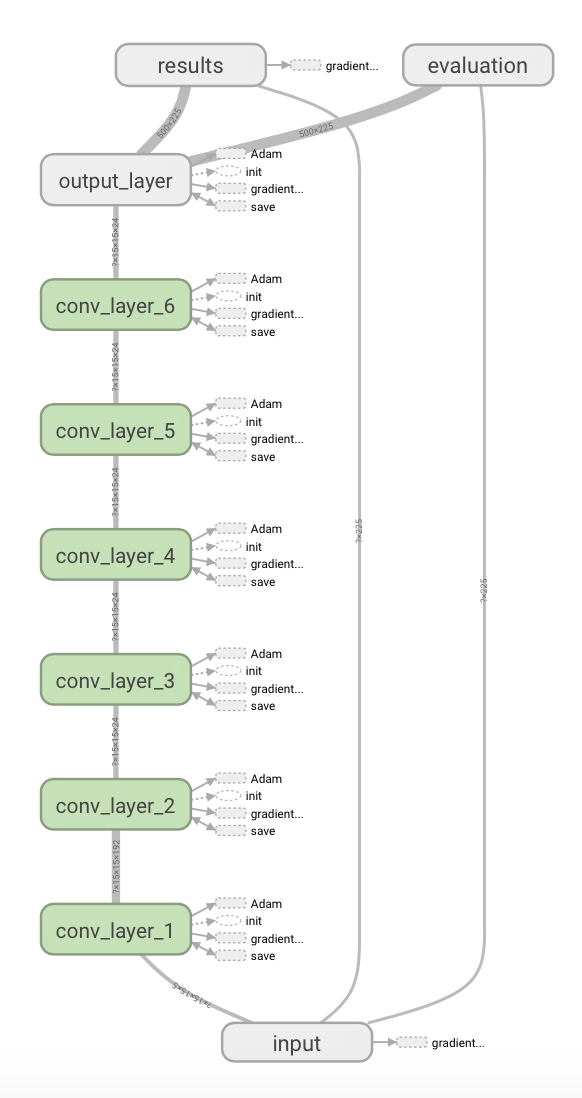
\includegraphics [height=8cm]{network}
\caption{CNN结构}
\label{network}
\end{center}

我们的神经网络的结构如图\ref{network}所示, 一共有8层, 可以看成一个convolutional neural network, 具体各层参数如下: 

\begin{itemize}
	\item \textbf{Input Layer}: $15 \times 15 \times 5$ 的提取的特征, 分为5个slice, 每一个slice是一个$15 \times 15$的矩阵$A$,$a_{i,j}$存储$(i, j)$这个位置的信息, 并且只有0/1两个取值, 5个slice 存储的信息分别是: 全1/全0/是否是我的子/是否是对方的子/是否是空. 这样的特征是非常原始的, 但是由于CNN在特征提取方面的能力, 即使非常原始的特征也能取得很好的效果. 
	\item \textbf{Hidden Layer 1}: $S = 1$ (Stride), $F = 5$ (Receptive Field), $P = 2$ (Zero Padding), filter: $5 \times 5 \times 5 \times k$,激励函数是relu, 一层的cube是$15 \times 15 \times k$
	\item \textbf{Hidden Layer 2 - 6}: $S = 1$, $F = 3$, $P = 2$, filter: $3 \times 3 \times k' \times k'$(第2层是$3 \times 3 \times k \times k'$),激励函数是relu, 一层的cube是$15 \times 15 \times k'$
	\item \textbf{Output Layer}: 第7层到Output Layer之间的连接用Softmax,$15 \times 15$ 的概率分布.
\end{itemize}

我们尝试了多组$(k, k')$, 最后选择了$k = 81$, $k' = 24$.

\noindent \textbf{SL policy network $\bm{p_\sigma}$: Training}

在训练的时候, 我们黑白分别训练, 把数据集分成训练集, 交叉验证集和测试集三个部分,每个数据包含了输入(棋盘局势$s$)和标记(人类选手的走棋选择$a$). 对于白棋分别是218853(训练集), 60000(交叉验证集), 60000(测试集); 黑棋分别是206701(训练集), 60000(交叉验证集), 60000(测试集).

在训练的时候, 每一步, 随机选择从训练集中选择$m$个样本$\{s^i, a^i\}_{i=1}^m$,使用随机梯度下降法来训练,最小化交叉熵,令梯度为: 

\[
\Delta\sigma = \frac{\alpha}{m} \sum_{i=1}^{m} \frac{\partial\log p_\sigma(a^i|s^i)}{\partial \sigma}
\]

学习速率$\alpha$一开始为$0.003$并且训练$2 \times 10^4$步减少一半, 一共训练了$2 \times 10^5$步,mini-batch size $m = 100$, 最后各自的准确度分别是$54.1\%$(黑)$48.5\%$(白).

\subsection{Greedy Policy Oracle}

\textcolor[rgb]{1,0,0}{xy补全}

\subsection{Reinforcement Learning of Policy Networks}

\noindent \textbf{RL policy network $\bm{p_\rho}$: Architecture}

我们采取和$p_\sigma$一样的结构, 同样黑白分别创建一个网络.

\noindent \textbf{RL policy network $\bm{p_\rho}$: Training}

训练对于黑白同时展开,对于黑/白的每一步训练,mini-batch并行地进行了$n=16$场对决.每场对决都是在当前的参数$\rho$和在对手池中的之前的某个参数$\rho'$展开.一开始全部是$\sigma$,每训练2次,就把当前的参数$\rho$放到对手池里.

每次更新的梯度如下:

\[
\Delta\rho = \frac{\alpha}{n} \sum_{i=1}^n\sum_{t=1}^{T_i} \frac{\partial\log p_\rho(a_t^i|s_t^i)}{\partial \rho}(z_t^i-v(s_t^i))
\]

在对决的时候,为了增加其不确定性,从而增强他的学习能力,对于每一个状态$s$,我们并不一定取$p_\rho(a|s)$最大的那个$a$,而是求出$p_\rho(\cdot|s)$的分布,然后在$[0,1)$中随机一个数,看他落在哪个$a$的分布里面,就选择哪个$a$.

最后我们统计了他和最初的$p_\sigma$按概率分布对决的胜率,为$77\%$(黑), $81\%$(白).

\subsection{Value Networks}

\noindent \textbf{Value networks $\bm{v_\theta}$: Architecture}

value network $v_\theta$的结构和$p_\sigma$基本一致

\begin{itemize}
	\item \textbf{Input Layer}: $15 \times 15 \times 5$ 的提取的特征, 意义同
	\item \textbf{Hidden Layer 1}: $S = 1$ (Stride), $F = 5$ (Receptive Field), $P = 2$ (Zero Padding), filter: $5 \times 5 \times 5 \times k$,激励函数是relu, 一层的cube是$15 \times 15 \times k$
	\item \textbf{Hidden Layer 2 - 6}: $S = 1$, $F = 3$, $P = 2$, filter: $3 \times 3 \times k' \times k'$(第2层是$3 \times 3 \times k \times k'$), 激励函数是relu, 一层的cube是$15 \times 15 \times k'$
	\item \textbf{Hidden Layer 7}: $S = 1$, $F = 1$, $P = 0$, filter: $1 \times 1 \times k \times k'$, 最后在reshape成一个$225$个节点的层, 激励函数是relu. 
	\item \textbf{Hidden Layer 8}: 第7层到第8层是全连接, 激励函数是relu.
	\item \textbf{Output Layer}: 第8层到Output Layer之间的连接用tanh,最后生成一个$[-1,1]$的整数表示己方获胜的概率.
\end{itemize}

\noindent \textbf{Value network $\bm{p_\rho}$: Training}

数据集来自于用$p_\sigma$和$p_\rho$创建的$3 \times 10^5$组人工数据.

对于每个数据,执行以下几步

\begin{itemize}
	\item 随机一个数$U$(1 - 60),前$U-1$步都用$p_\sigma$走
	\item 第$U$步随机走(随机找一个合法的)
	\item 接下来都用$p_\rho$走,一直走到完,算出$z_T$.
	\item 把$(s_{U+1}, z_{U+1})$放入数据集
\end{itemize}

最后最小化均方差, 梯度如下: 
\[
\Delta\theta = \frac{\alpha}{m} \sum_{i=1}^m\frac{\partial v_\theta(s^i)}{\partial \theta}(z^i - v_\theta(s^i))
\]

\textcolor[rgb]{1,0,0}{具体的训练效果}

\section{Tree Search Algorithm}

\subsection{Overview}

我们采用Monte Carlo tree search作为主要算法.

考虑Monte Carlo tree上的每一个点,都表示一个棋局的状态$s$,每条边都可以用$(s, a)$来表示,其中$a$是一个合法的走棋,Monte Carlo tree search的算法分为4个部分.

\noindent\textbf{Selection}: 对于当前的点,如果不是叶子节点,考虑下一步的sampling该选哪一步,基于UCT算法的改良,我们选择$Q(s, a) + u(s, a)$最大的那个,一直往下走到叶子节点$s_L$\textbf{(注意此时这个节点还不在树中,但是这个节点的父亲在树中)}为止.其中$u(s, a) = c_{puct}P(s, a)\frac{\sum_{b}N(s,b)}{1+N(s,a)}$,$P(s, a)=p_\sigma(a|s)$ 用SL Policy Network $p_\sigma$来算,$N(s,a)$表示$(s,a)$这条边参加sampling的次数.

\noindent\textbf{Evaluation}: 从叶子节点$s_L$开始,接下来用$p_\pi$来模拟双方落子行为,算出最后的输赢情况$z_L$,然后计算出叶子节点在这一轮模拟中的值$V(s_L^i)=(1-\lambda)v_\theta(s_L) + \lambda z_L$.

\noindent\textbf{Backup}: 向上更新所有的祖先的$Q$值和$N$值.其中$N(s, a) = \sum_{i=1}^n[(s,a,i)]$,$Q(s, a) = \frac{1}{N(s,a)}\sum_{i=1}^n{[(s,a,i)] \cdot V(s_L^i)}$,其中$[(s,a,i)]$为$1$当且仅当在第$i$轮模拟中经过了$(s, a)$这条边.

\noindent\textbf{Expansion}: 如果某条边$(s, a)$的访问次数超过了阀值,就把$s'= f(s,a)$加入到搜索树中来,$f(s,a)$表示这个边连向的某个儿子.

在搜索完成之后,我们的AI会选择走$N(s, a)$最大的那个$a$,保留$s'=f(s, a)$子树的内容,然后释放其他所有节点的内存.

\subsection{Implementation Details}

\underline{具体实现中为了加快速度可以使用多线程},在MCTS中的每个节点$s$都包含由\textbf{所有}合法操作$a$组成的边$(s,a)$,对于每条边,都需要记录一下数据:

\begin{itemize}
	\item $P(s, a)$ 即Overview中的$P(s, a)$
	\item $N_v(s, a)$ 即Overview中的$N(s, a)$,这里细化指的是在这棵子树中计算过的$v_\theta(s)$的次数.
	\item $N_r(s, a)$ 即Overview中的$N(s, a)$,这里细化指的是在这棵子树中计算过的rollout的次数.
	\item $W_v(s, a)$ 指的是在这棵子树中计算过的$v_\theta(s)$的和.
	\item $W_r(s, a)$ 指的是在这棵子树中计算过的rollout的$z_L$的和.
\end{itemize}

\noindent\textbf{Selection}

每次从根开始往下搜索,直到走到一个叶子节点为止(设这时候的时间为L),对于所有的$t < L$,令$a_t = argmax_a(Q(s_t, a) + u(s_t, a))$,其中$u(s, a) = c_{puct}P(s, a)\frac{\sqrt{\sum_{b}N(s,b)}}{1+N(s,a)}$,$c_{puct}$是一个参数,最后被定为$5$.

\noindent\textbf{Evaluation}

把叶子节点$s_L$放到队列中计算$v_\theta(s_L)$(这里采用多线程,并且可以加一个记忆化).对于rollout,下棋双方都用$p_\pi$来模拟,也采用多线程放在队列里依次处理.

\noindent\textbf{Backup}

考虑这次模拟对所有树中边的影响,我们分别更新rollout的值$N_r(s, a), W_r(s, a)$和value network的值$N_v(s, a), W_v(s, a)$,最后更新$Q(s, a)$的值

\[
Q(s, a) = (1 - \lambda)\frac{W_v(s,a)}{N_v(s,a)}+\lambda\frac{W_r(s,a)}{N_v(s,a)}
\]

AlphaGo 中 $\lambda=0.5$的时候效果最好. \textcolor[rgb]{1,0,0}{我们的还在测试中.}

分别考虑rollout和value network的更新

\begin{itemize}
	\item 对rollout更新的时候,每次把某个节点塞到队列里面计算的时候,就把所有相关的$N_r(s,a)$和$W_r(s,a)$进行修改:$N_r(s,a)=N_r(s,a)+n_{vl}$, $W_r(s,a)=W_r(s,a)-n_{vl}$,让他看起来输了$n_{vl}$场防止多次运算,最后计算出来的时候让$N_r(s,a)=N_r(s,a)-n_{vl}+1$, $W_r(s,a)=W_r(s,a)+n_{vl}+z_L$.
	\item 对value network进行更新的时候,算出来之后更新所有相关的边$N_v(s,a)=N_v(s,a)+1$,$W_v(s,a)=W_v(s,a)+v_\theta(s_L)$.
\end{itemize}

这里$n_{vl}$取$3$.

\noindent\textbf{Expansion}

当一条边$(s, a)$的访问次数超过一个阀值$n_{thr}$的时候,就把后续的状态$s'=f(s,a)$加入到树中,把这个节点的所有边都初始化: $N_v(s',a)=N_r(s',a)=0$,$W_v(s',a)=W_r(s',a)=0$, $P(s',a)=p_\sigma(a|s')$,具体计算的时候$P(s',a)=p_\sigma(a|s')$这步运算也采用多线程,一开始先用tree policy来计算$P(s',a)$(tree policy和rollout policy类似,但是拥有更多的特征值),直到$p_\sigma(a|s')$计算完成之后再让$P(s',a)=p_\sigma^\beta(a|s')$,这里softmax temperature被设为$\beta$,$\beta$取$0.67$,$n_{thr}$需要与实际队列的情况相契合.

\section{System Architecture}

\section{User Interface}

\section{Data Flow}

\begin{thebibliography}{1}
\bibitem{alphago}
Silver, David, et al. Mastering the game of Go with deep neural networks and tree search, Nature 529.7587: 484-489, 2016
\bibitem{renjunet}
http://renju.net/downloads/downloads.php, 2015
\end{thebibliography}

\end{document}

